\subsection{Coxeter arrangements in \texorpdfstring{$\Hbb^3$}{H3}}

Since the second half of the 1st semester, I have been investigating Coxeter arrangements of rank 3 and 4 Coxeter groups of hyperbolic signature.
The nature of this investigation has been informed by the fact that a lot of progress in this field has been made by looking at relevant pictures.
Accordingly, I have developed a set of tools to visualise Coxeter arrangements in $\Hbb^2$ and $\Hbb^3$ using Mathematica.
Developing such tools also has the advantage of providing tangible examples on which to try ideas, and was a good way to learn hyperbolic geometry.
In the following, let $G_{353}$ and $G_{555}$ be Coxeter groups corresponding to the following $\Gamma$.
\[
	G_{353} \leftrightsquigarrow
	\begin{tikzpicture}
		\def\size{0.7}
		\tikzstyle{every label}=[font=\footnotesize]
		\tikzstyle{every node}=[font=\footnotesize]

		% First square nodes
		\node[FSC] (l)	at (0,0)	{};
		\node[FSC] (ml)	at ($(l)+(\size,0)$)	{};
		\node[FSC] (mr)	at ($(ml)+(\size,0)$)	{};
		\node[FSC] (r)	at ($(mr)+(\size,0)$)	{};

		\draw (l) to node[above] {3} (ml);
		\draw (ml) to node[above] {5} (mr);
		\draw (mr) to node[above] {3} (r);
	\end{tikzpicture}\;,
	\quad
	\quad
	G_{555} \leftrightsquigarrow
	\begin{tikzpicture}[baseline={(c.base)}]
		\def\size{0.7}
		\tikzstyle{every label}=[font=\footnotesize]
		\tikzstyle{every node}=[font=\footnotesize]

		% First square nodes
		\node[FSC] (c)	at (0,0)	{};
		\node[FSC] (t)	at ($(c)+(0,\size)$)	{};
		\node[FSC] (r)	at ($(c)+(0.83*\size,-0.83*\size)$)	{};
		\node[FSC] (l)	at ($(c)+(-0.83*\size,-0.83*\size)$)	{};

		\draw (c) to node[left] {5} (t);
		\draw (c) to node[right, near start] {5} (r);
		\draw (c) to node[left, near start] {5} (l);
	\end{tikzpicture}
\]

It turns out that $G_{353}$ is the only rank 4 Coxeter system for which the $K(\pi,1)$ conjecture is open.
It also happens to be geometrically well-behaved, in that its fundamental domain in $\Hbb^3$ is compact and of finite volume.

The geometry of a rank 4 hyperbolic Coxeter group is determined by 6 interplanar angles.
In Euclidean space, if these interplanar angles do correspond to some tetrahedron, then it is relatively simple to find a specific tetrahedron that realises these angles.
In $\Hbb^3$, this is more complicated, since angles are specific scale.
We developed a way to symbolically compute tetrahedrons in $\Hbb^3$ corresponding to any appropriate Coxeter group.

We used this to realise a specific model for $G_{353}$.
In \cref{fig:353_origin}, we show 120  cells (many of which are at the back of the plot and not visible) in the Coxeter arrangement for $G_{353}$ that have a vertex at the origin.
The chosen fundamental chamber has an edge along the $z$-axis in blue.
The faces of the fundamental chamber were coloured red, green, blue and orange, and we considered the Coxeter element that corresponded to the product of those faces in that order.
The edges of the fundamental chamber were also coloured in a unique way.
In \cref{fig:353_origin}, we only see orange faces since the cells shown are the orbit under the subgroup generated by the red, green and blue faces of the fundamental chamber, and we see 120 cells because that is the order of that parabolic subgroup.

\begin{figure}
	\centering
	\begin{subfigure}[t]{.45\textwidth}
		\centering
		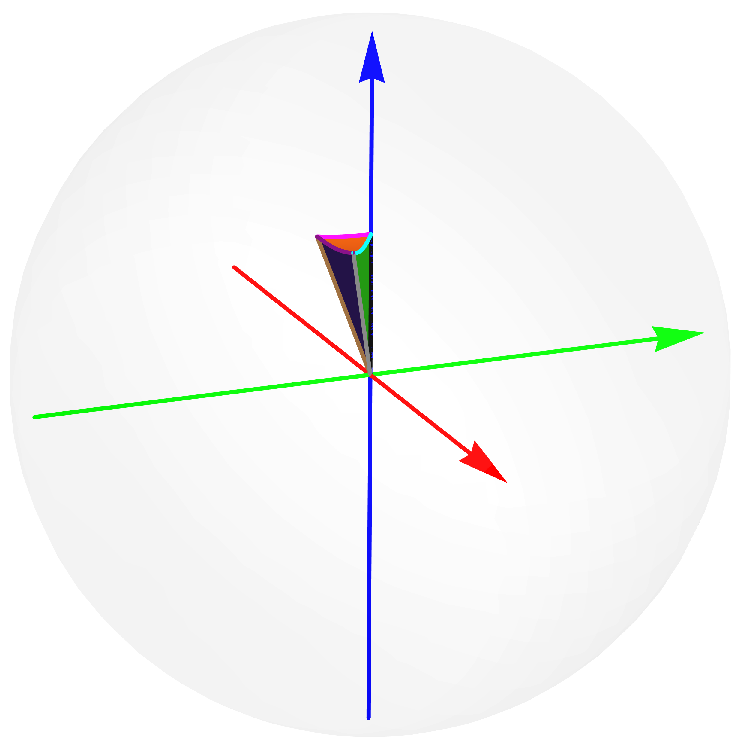
\includegraphics[width=6cm]{353_fundchamber.pdf}
		\caption{Our chosen fundamental chamber for $G_{353}$.}
		\label{fig:353_fund_chamber}
	\end{subfigure}
	\hspace{0.2ex}
	\begin{subfigure}[t]{.45\textwidth}
		\centering
		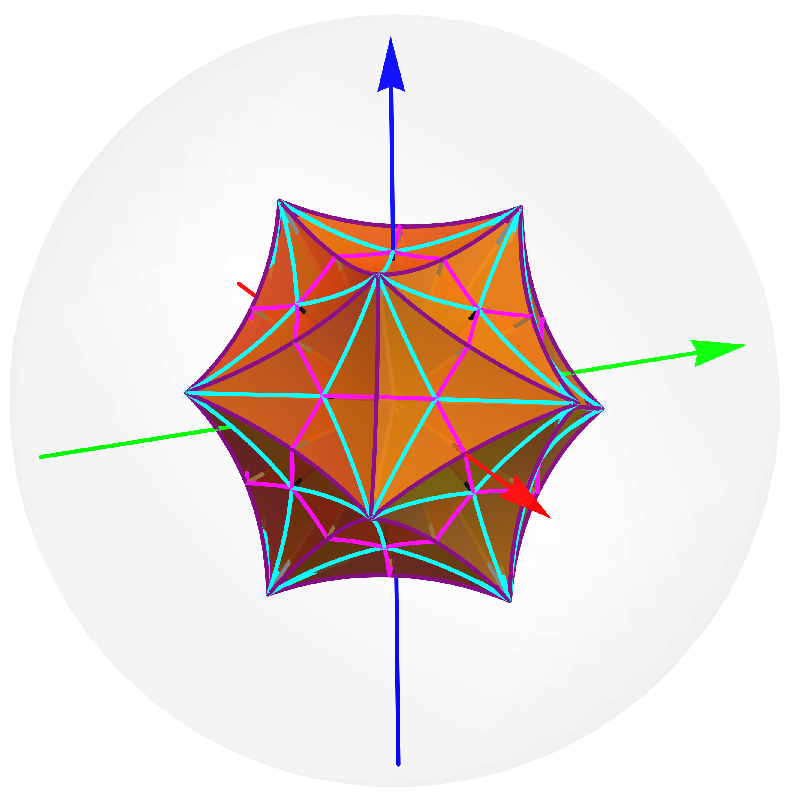
\includegraphics[width=6cm]{353_origin.pdf}
		\caption{A part of the Coxeter arrangement for $G_{353}$ consisting of 120 copies of the fundamental chamber that are positioned at the origin.}
		\label{fig:353_origin}
	\end{subfigure}%
	\caption{Realising the Coxeter arrangement for $G_{353}$.}
	\label{fig:test}
\end{figure}

In \cref{fig:353_cut}, we see a cut of the Coxeter arrangement of $G_{353}$ along a plane in  $\Hbb^3$.
For this, we initially plotted significantly more cells of the Coxeter arrangement than in  \cref{fig:353_origin}.
This is an irregular tiling of $\Hbb^2$.
In the case of  $G_{353}$, taking different cuts reveals the same tiling up to translation.

In \cref{fig:353_coxeter_axis}, we see the Coxeter axis corresponding to the product of the red, green, blue and orange planes of the fundamental chamber in that order.
Alongside this, we see some cells that lie along the Coxeter axis.
Such cells are important as any reflection factorisation of a Coxeter element that makes a tetrahedron must be one of these cells.

\begin{figure}
	\centering
	\begin{minipage}{.5\textwidth}
		\centering
		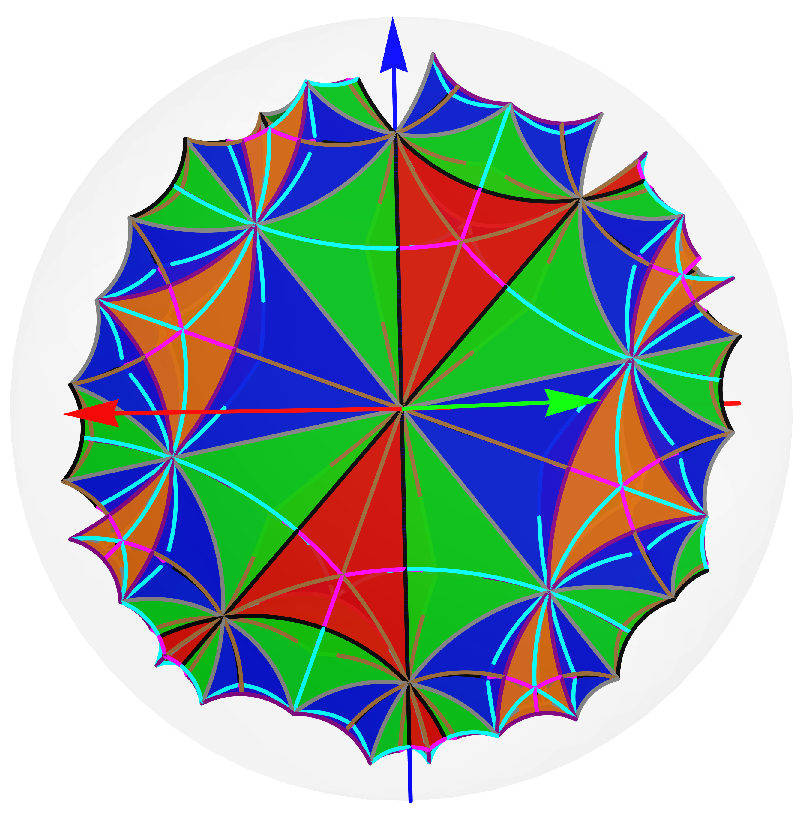
\includegraphics[width=6cm]{353_cut.pdf}
		\caption{A cut of the Coxeter arrangement of $G_{353}$ along a plane in $\Hbb^3$.}
		\label{fig:353_cut}
	\end{minipage}%
	\begin{minipage}{.5\textwidth}
		\centering
		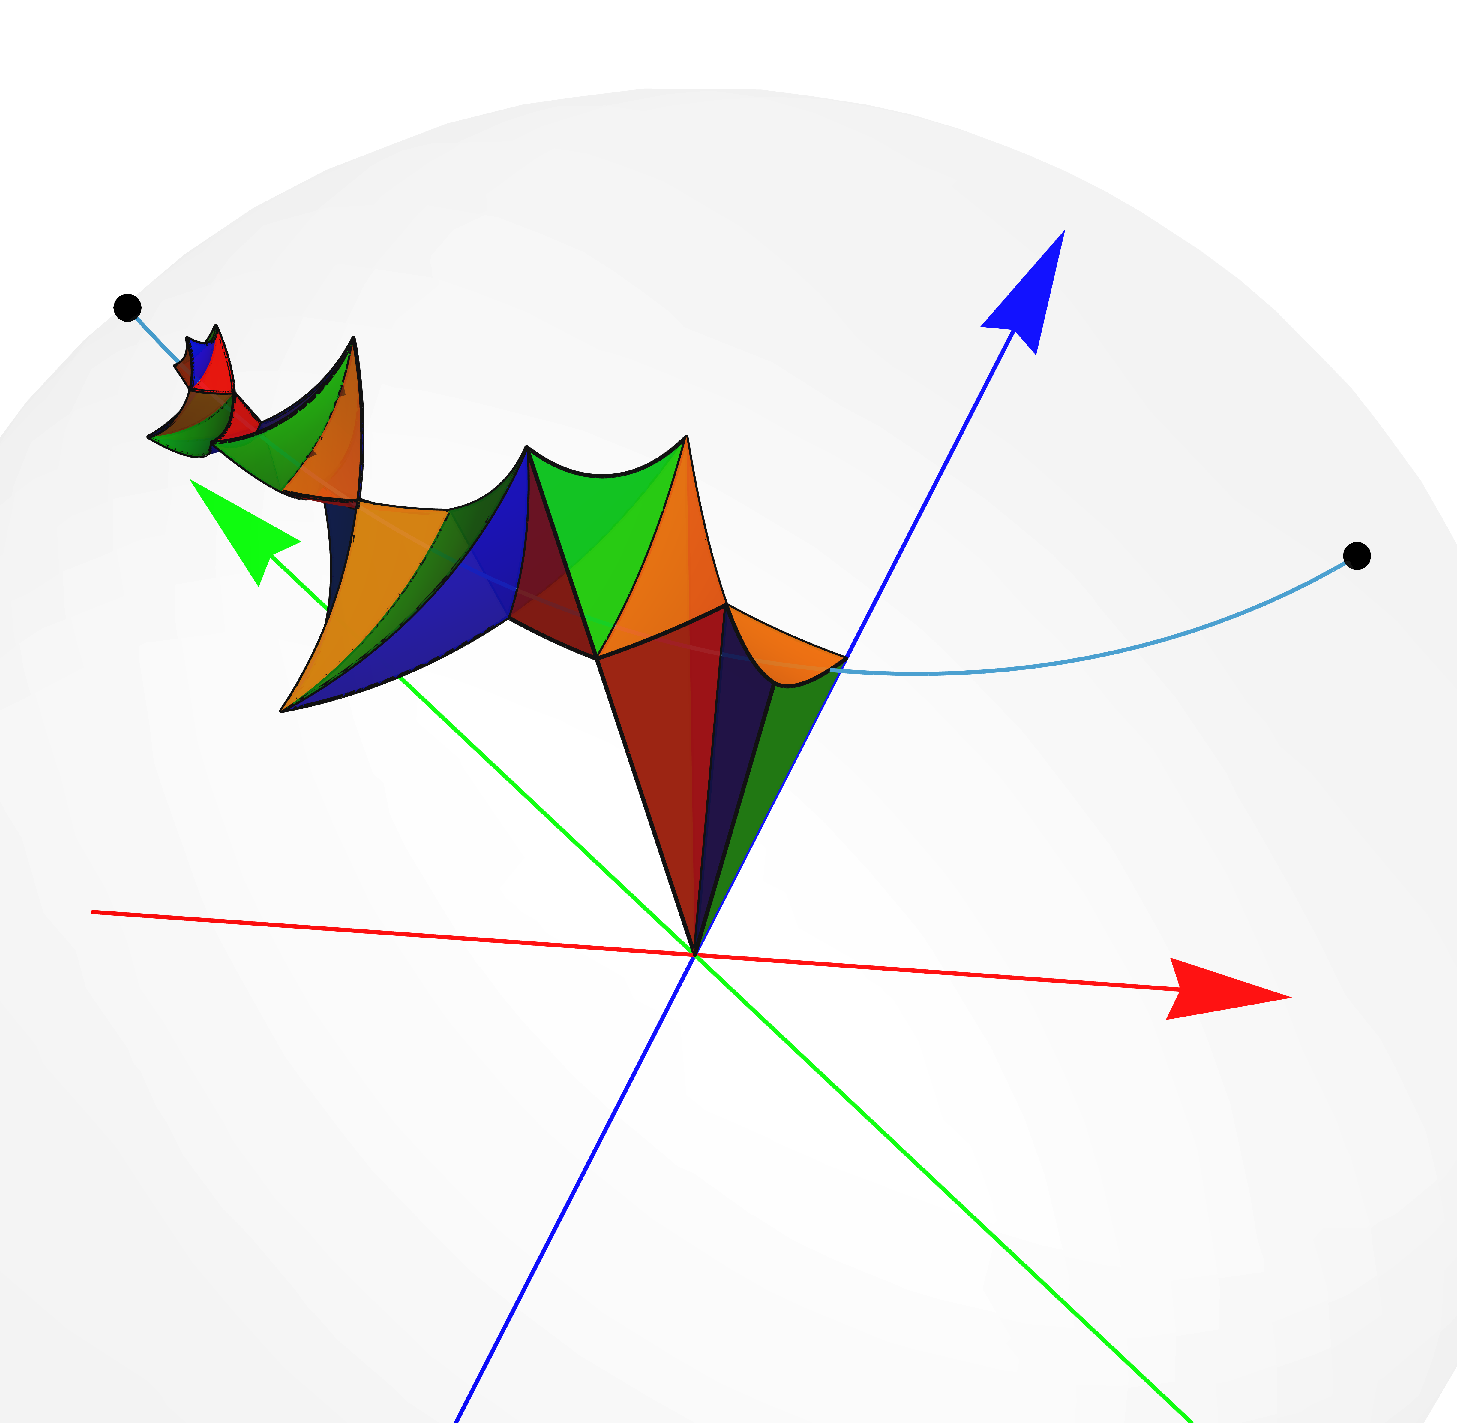
\includegraphics[width=6cm]{353_coxeteraxis.pdf}
		\caption{The Coxeter axis Corresponding to a Coxeter element in $G_{353}$, as well as some cells that lie along this Coxeter axis.}
		\label{fig:353_coxeter_axis}
	\end{minipage}
\end{figure}

We were not able to use these tools to prove anything about $G_{353}$, but in developing these plots and the geometric tools needed to make them, I gained a lot of intuition and knowledge for these hyperbolic arrangements.
We were also able to compute some closed forms for certain geometric constructions in $\Hbb^2$ and  $\Hbb^3$ useful for future calculations.
For example, we may denote planes in $\Hbb^3$ as $p = (\mathbf{n},r)$, where $\mathbf{n}$ and $r$ are a normal vector and non-negative real respectively, such that the circle of intersection of $p$ with the unit sphere is the same as the circle of intersection of the plane $\mathbf{n} \cdot \mathbf{x} = r$ with the unit sphere.
In this notation, the reflection of the plane $p_1 =(\mathbf{n_1},r)$ through $p_2 = (\mathbf{n_2},s)$ with $\mathbf{n_1}=(x,y,z)$ and  $\mathbf{n_2}=(a,b,c)$ is
\begin{align*}
	 & {\scriptscriptstyle R_{p_2}(p_1) =\bigg(\text{Sign}\left(r(1+s^2)-2s(\mathbf{n_1}\cdot\mathbf{n_2})\right)\; \text{Normalise}\big[}                      \\
	 & {\scriptscriptstyle\quad 2ars + (1-s^2)x-2(a^2x+aby+acz),                                                                                             }  \\
	 & {\scriptscriptstyle\quad 2brs + (1-s^2)y-2(b^2y+abx+bcz),                                                                                             }  \\
	 & {\scriptscriptstyle\quad 2crs + (1-s^2)z-2(c^2z+acx+bcy) \;\big],                                                                                      } \\
	 & {\scriptscriptstyle\sqrt{\frac{r^2 (1 + s^2)^2 - 4 r s (1 + s^2) (\mathbf{n_1}\cdot\mathbf{n_2}) +
					4 s^2 ((-1 + c^2) (-1 + y^2) + 2 a c x z + (-1 + 2 c^2) z^2 +
					2 b y (a x + c z) + b^2 (-1 + 2 y^2 + z^2))}{1 + s^4 -
					4 r s (\mathbf{n_1}\cdot\mathbf{n_2}) - 4 r s^3 (\mathbf{n_1}\cdot\mathbf{n_2}) +
					s^2 (2 + 4 r^2 - 4 y^2 + 8 a c x z - 4 z^2 + 8 b y (a x + c z) +
					4 b^2 (-1 + 2 y^2 + z^2) + 4 c^2 (-1 + y^2 + 2 z^2))}}\,\bigg)}.
\end{align*}

We also investigated Coxeter arrangements where the fundamental domain was of infinite volume.
For $\Gamma$ of hyperbolic signature, this can only happen in rank 4 or greater.
This is because in  $\Hbb^n$ for  $n\geq 3$, a simplex can have well-defined interplanar angles, but have vertices ``poking out" beyond infinity, as shown in \cref{fig:555_orthogonal_planes}.

Coxeter systems of hyperbolic signature, where the fundamental chamber is compact or of finite volume are more well understood, and classified in \cite[Section 6.9]{humphreys_reflection_1990}.

Despite being less well classified, these groups have interesting properties not shared by limit sets, as shown in \cref{fig:555_limitset}.
The limit set is the set of points in $\Hbb^3$ that a generic point will tend to by random action by the group.
Such limit sets are of general interest in Kleinian groups (groups with a $\Hbb^3$ action).
Parabolic subgroups corresponding to triples of generators act on the plane that is mutually orthogonal to the triple.
The action of the triple on this plane is some hyperbolic rank 3 Coxeter group action on $\Hbb^2$ (in this case, the $(2,5,5)$ triangle group), so its limit set is the boundary at infinity (of this copy of $\Hbb^2$).
This limit set represents a lower dimensional object of symmetry of such a group.

Furthermore, using and extending work of McMullen \cite{mcmullen_coxeter_2002}, we constructed a different metric space on which such Coxeter groups act.
This is constructed by naively extending tetrahedrons beyond the unit ball in the Klein model, shown for $G_{555}$ in \cref{fig:555_exteded_space}.
This gives a subspace of $\E^3$, and we place the so-called Hilbert metric on this space, which is different from any of the usual hyperbolic metrics inside the unit sphere.
We call this space $\Omega_\Gamma$.
When a hyperbolic signature Coxeter group has cofinite volume, then this space ends up being canonically isometric to  $\Hbb^3$.
See \cite{papadopoulos_troyanov_handbook_2014} for an introduction to the Hilbert metric.

\begin{figure}
	\centering
	\begin{subfigure}[t]{.45\textwidth}
		\centering
		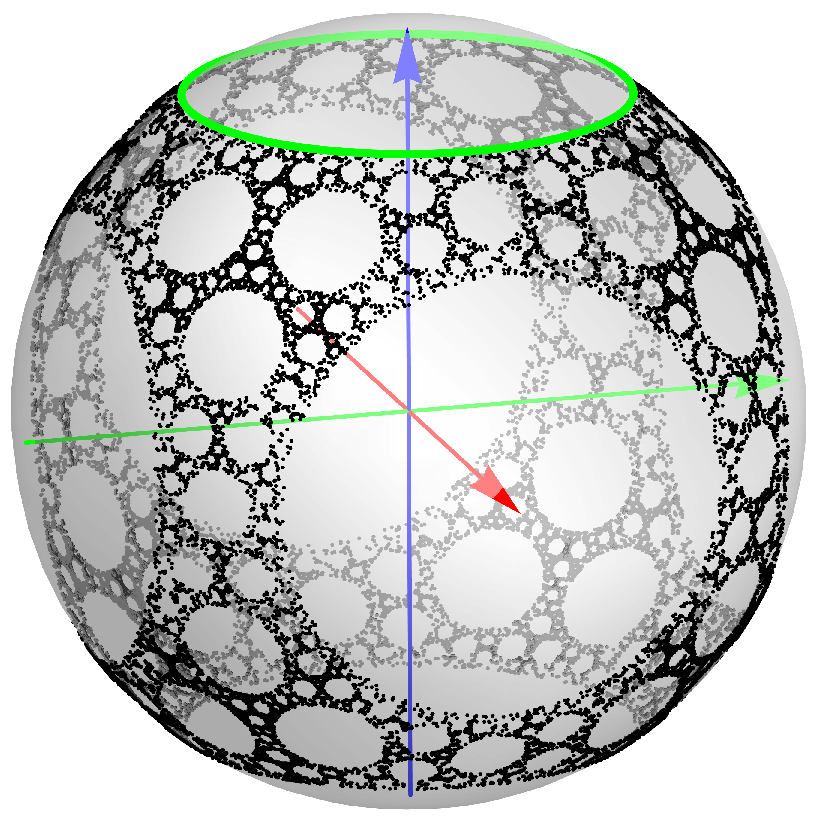
\includegraphics[width=6cm]{555_limitset.pdf}
		\caption{The limit set of $G_{555}$.}
		\label{fig:555_limitset}
	\end{subfigure}
	\hspace{0.2ex}
	\begin{subfigure}[t]{.45\textwidth}
		\centering
		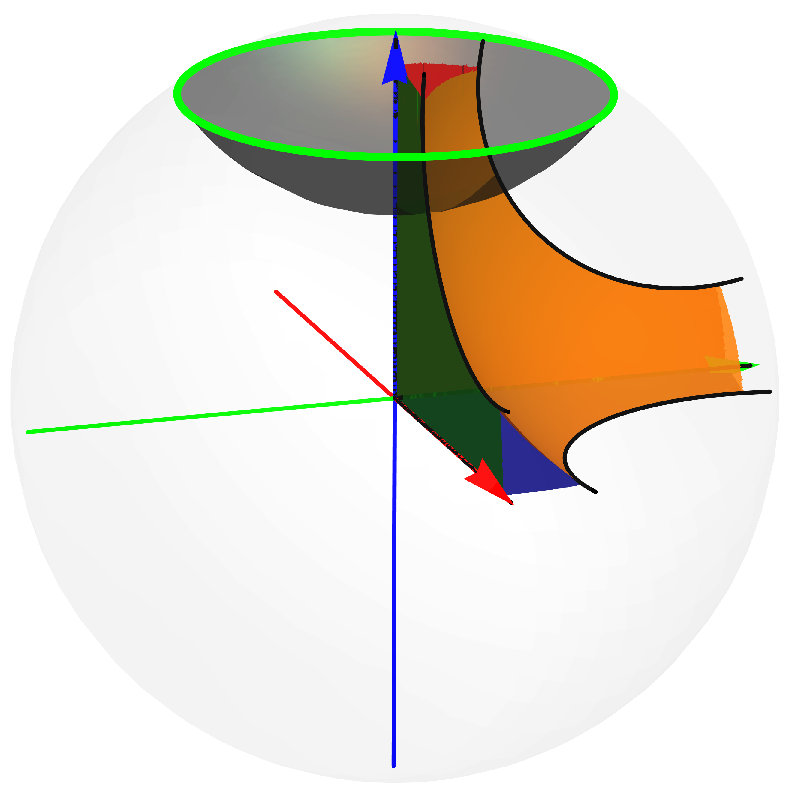
\includegraphics[width=6cm]{555_orthplanes.pdf}
		\caption{A fundamental chamber of $G_{555}$ drawn with coloured planes.
			A plane orthogonal to three planes of the fundamental chamber (in black) defines a circle seen in the limit set.}
		\label{fig:555_orthogonal_planes}
	\end{subfigure}%
	\caption{Exploring the limit set of $G_{555}$.}
\end{figure}

\begin{figure}
	\centering
	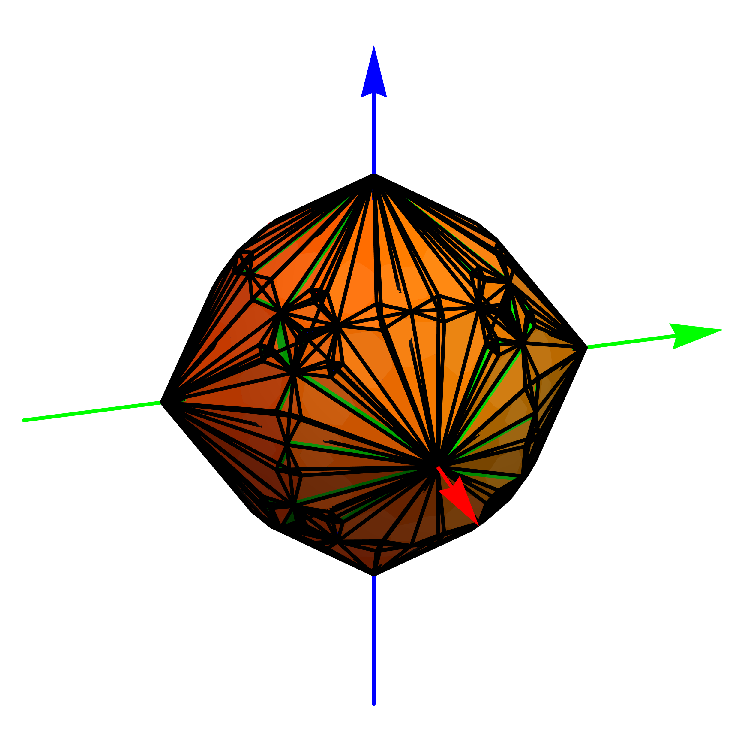
\includegraphics[width=7cm]{555_extended.pdf}
	\caption{A rough approximation of $\Omega_\Gamma$ for $G_{555}$.}
	\label{fig:555_exteded_space}
\end{figure}


It can be shown that the Coxeter group acts by isometries on $\Omega_\Gamma$, and this construction works for any Coxeter system with hyperbolic signature and infinite co-volume.
Using these two metrics, it can be shown that if a geodesic in $\Hbb^n$ is preserved setwise, and moved by translation by some element of the Coxeter group (in particular, the Coxeter axis satisfies this), then this line meets the boundary at two points where the boundary of $\Omega_\Gamma$ meets the unit sphere.
Such points are points in the limit set.
In the case of $G_{555}$, a choice of Coxeter element has axis from  $\frac{1}{\sqrt{3}}(1,1,1)$ to $\frac{1}{\sqrt{3}}(-1,-1,-1)$.


